%%%%%%%%%%%%%%%%%%%%%%%%%%%%%%%%%%%%%%%%%%%%%%%%%%%%%%%%%%%%%%%%%%%%%%%%%%%%
% Section 3: Getting Started
%	This section contains installation instructions for RapidSmith2, and
%	how to test the installation is correct. 
%%%%%%%%%%%%%%%%%%%%%%%%%%%%%%%%%%%%%%%%%%%%%%%%%%%%%%%%%%%%%%%%%%%%%%%%%%%%
\newpage
\section{Getting Started}
\graphicspath{{./techReportFigures/sec3_gettingStarted/}}

\subsection{Installation}

RapidSmith2 is available on Github at:
{\color{blue}{\url{https://github.com/byuccl/RapidSmith2}}}.
You can either build RapidSmith2 into .class and .jar files for use in any Java
environment, or configure RapidSmith2 to work in an IDE (recommended).

\subsubsection{Requirements for Installation and Use}
\begin{itemize}
  \item Windows, Linux or Mac OS X all will work (see additional notes below for
  Mac OS X)
  \item Vivado 2016.2. Later versions of Vivado may work, have not been tested
  yet. Earlier versions will not work.
  \item JDK 1.8 or later
  \item Tincr 
\end{itemize}

Tincr is a companion project
({\color{blue}{\url{https://github.com/byuccl/tincr}}}) which is used for
importing/exporting designs between Vivado and RapidSmith2. Installation
instructions for Tincr can be found at the repository linked above. For getting
started (running the example programs on the provided sample designs) you will
not need it installed. Later, as you  actually start processing your own Vivado
designs you will need to obtain and install it. There are additional
dependencies beyond these required for installation, but they are either
provided in the distribution itself or are automatically retrieved for you as a
part of the installation process. Examples of these additional dependencies
include QT Jambi and the BYU Edif Tools.
 
\subsubsection{Steps for Installation}

\begin{enumerate}
  \item Clone the RapidSmith2 repository at
  {\color{blue}{\url{https://github.com/byuccl/RapidSmith2}}}. If you are not
  familiar with GitHub, you will need to install Git on your computer, and run the
  following command in an open terminal: 

\begin{lstlisting} [numbers=none,keywordstyle=\ttfamily,commentstyle=\color{black}] 
   git clone https://github.com/byuccl/RapidSmith2
\end{lstlisting}
 
  \noindent This will copy the RapidSmith2 repository into a local directory.
  \item Create a new environment variable called RAPIDSMITH\_PATH, and point it
  to your local repository of RapidSmith2 that you setup in step (1). This is needed so
  RapidSmith2 can find required device files and other items at runtime.
  \item Build the  RapidSmith2 project. RapidSmith2 is managed using a gradle build system.
  To build the project, navigate to your local repository of RapidSmith2 and execute one
  of the following scripts in a terminal:
  
\begin{lstlisting} [numbers=none,keywordstyle=\ttfamily]
	./gradlew build (unix)
	gradlew.bat build (windows)
\end{lstlisting}
  
  The build process could take a few minutes.
  \item At this point, you have two choices: set up RapidSmith2 for use in an IDE, or
  run RapidSmith2 from the command line. Both choices are detailed below.
  \paragraph{Running from an IDE} The gradle scripts in RapidSmith2 currently support
  setup for both Eclipse and IDEA Java IDEs. This section will detail how to
  setup the Eclipse environment, but similar steps can be taken for IDEA. If
  using Eclipse, it is best to use version Eclipse Neon or later. To create a
  new eclipse project, execute one of the following in a terminal:
  
\begin{lstlisting} [numbers=none,keywordstyle=\ttfamily]
	gradlew antlr eclipse (unix)       
	gradlew.bat antlr eclipse (windows)
\end{lstlisting}
  
  Executing these will create an Eclipse \fil{.project} file. After the project
  file has been created, you can import the project into Eclipse by opening
  Eclipse and selecting:
  
\begin{lstlisting} [numbers=none,keywordstyle=\ttfamily]
	File->Open Projects From File System 
\end{lstlisting}
  
  and pointing it to your RapidSmith2 local repository. All Java source files
  will be found under \dir{src/main/java}. \pgm{NOTE:} Your RapidSmith2 git repository
  should not be put inside your eclipse workspace. It is better to put it
  elsewhere, and then import it into your workspace.
  \paragraph{Building on the Command Line} After step (3) in the installation
  process, gradlew produces everything that you will need to run RapidSmith2 from the
  command line. The following directories are created: 
  \begin{itemize}
    \item \fil{build/classes/main}: This folder contains the RapidSmith2 class file
    directory tree.
    \item \fil{build/libs}: This folder contains a Jar file of the RapidSmith2 class
    files.
    \item \fil{build/distributions}: This folder has both .zip and .tar files
    with contains all Jars needed to run RapidSmith2 from the command line. This
    includes a full jar of the RapidSmith2 build alond with copies of dependency Jars
    (such as QT-Jambi).
  \end{itemize} 
  After adding the appropriate .class files or Jars to your \texttt{CLASSPATH},
  you should be able to run RapidSmith2 tools from the command line. If you make any
  changes to the RapidSmith2 code, you will have to rebuild before running the program
  again (Step 3). \pgm{CAUTION:} An obvious thing to try is to mix and match
  developing in Eclipse but then running the resulting apps from the command
  line. Just be aware that Eclipse puts its compiled .class files in very
  different places than where the gradle build process puts its .class and
  .jar files. Make sure you understand that before you try to combine these two
  build/execution methods. Our suggested approach is to choose one or the
  other, but not both.
\end{enumerate}

\subsubsection{Docker Support}

RapidSmith2 is also available as a Docker container. To painlessly set up a working RapidSmith2 environment, type:

\begin{lstlisting} [numbers=none,keywordstyle=\ttfamily]
	docker run -it byuccl/rapidsmith2
\end{lstlisting}

\noindent For more information about Docker, see the
\href{https://docs.docker.com/engine/getstarted/}{\color{blue}guide}.

\subsubsection{Additional Notes for Mac OS X Installation}

The instructions above require you to set the \env{RAPIDSMITH\_PATH}
environment variable.  If running from the command line, the environment
variables can be added to your \fil{.bash\_profile} file as in any other
UNIX-like system.  However, if using an IDE such as Eclipse you either need to
define the environment variable for every Run Configuration you create, or you
need to add the \env{RAPIDSMITH\_PATH} definition system-wide in OS X. This can
be done, but how to do so differs based on what OS X version you are running
(and seems to have changed a number of times over the years). Search the web for
instructions for how to do so if you desire. \pgm{Hint}: you will likely have
to edit some \fil{.plist} files.

\subsubsection{Running RapidSmith2 Programs}
Some points to keep in mind while configuring and running RapidSmith2 programs:
\begin{itemize}
  \item The RapidSmith2 code base contains a number of assertions which may be helpful  
  as you are developing code.  These are not enabled by default in Java.  To
  enable them, add \opt{-ea} as a VM argument.  This is highly recommended.
  \item If you are running on a Mac, when running RapidSmith2 programs that use Qt  (any
  of the built-in programs like \pgm{DeviceBrowser}) that are GUI-based, you
  will need to supply an extra JVM switch, \opt{-XstartOnFirstThread}.
  \item A common error when running RapidSmith2 programs is failing to have your
  \env{RAPIDSMITH\_PATH} defined.  If this is the case when you try to execute a
  program, an \texttt{EnvironmentException} will be thrown telling you that you
  forgot to set the variable.
  \item If you are running on Windows, only a 32-bit QT Jar file is included in
  the RapidSmith2 repository. This means that you will need to set your JRE to a 32-bit
  version when running the GUI programs. We are working on updating QT to the
  latest version, so this will no longer be an issue.
  \item For Linux command line usage, the \env{CLASSPATH} environment variable
  must point to both the full (uncompressed) RapidSmith2 jar in the \dir{build/distributions}
  folder as well as all the jar files in the \dir{/lib} subdirectory. An example
  \env{CLASSPATH} could look like this:
\begin{lstlisting} [numbers=none,keywordstyle=\ttfamily,commentstyle=\color{black}] 
	�  �  � RAPIDSMITH2-SNAPSHOT/*:RAPIDSMITH2-SNAPSHOT/lib/*
\end{lstlisting}
\end{itemize}

\subsubsection{Testing Your Installation}
\noindent At this point you can test your installation by executing the java
\pgm{DeviceBrowser} program: 

\begin{lstlisting} [numbers=none,keywordstyle=\ttfamily]
java edu.byu.ece.rapidSmith.device.browser.DeviceBrowser
\end{lstlisting} 

\noindent This can be done either from within Eclipse or from the command line,
depending on how you are running RapidSmith2 (if running under OS X be sure to provide the
\opt{-XstartOnFirstThread JVM argument}. If all goes well you should see a
graphical representation showing the details of a physical FPGA device as shown
in \autoref{fig:deviceBrowser}.  You may initially be zoomed far in and might
want to zoom out to see the entire chip layout.

\begin{figure}[H]
\centering
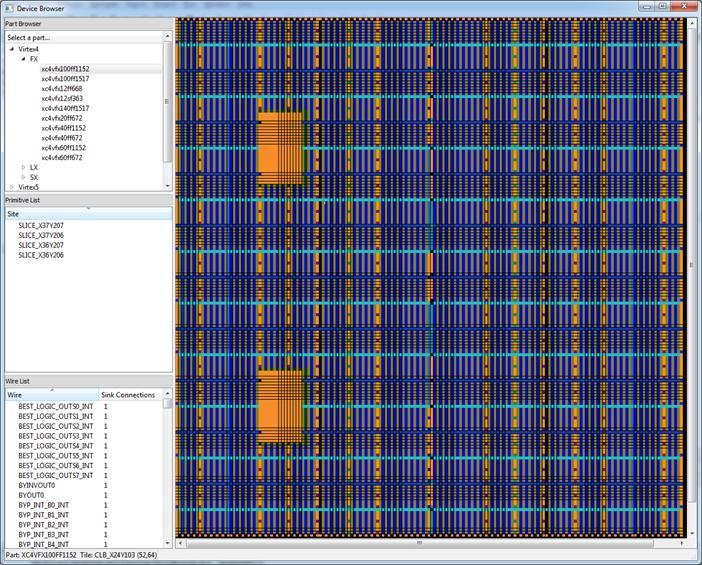
\includegraphics[width=0.8\columnwidth]{deviceBrowser.jpg}
\caption{\pgm{DeviceBrowser} Sample Display}
\label{fig:deviceBrowser}
\end{figure}

\subsection{Running Real Designs - An Overview}
This section will lead you through the required steps to export an implemented 
design from Vivado and load it into RapidSmith2. It will also demonstrate how to
export a modified design from RapidSmith2 back into Vivado to complete
implementation. Specifically, in this example you will fully synthesize, place,
and route a simple Vivado FPGA design using Tcl commands, and then export it to
RapidSmith2. As you gain more experience, you can choose to export designs from
Vivado post-synthesis, post-place, or post-route. You can also choose to export
and import designs that have been implemented ``out-of-context.'' The
steps to be covered in this tutorial include:

\begin{enumerate}
  \item Synthesize, place and route a design in Vivado
  \item  Export the design from Vivado in the form of an RSCP (RapidSmith
  Checkpoint)
  \item Import the RSCP  into RapidSmith2
  \item Run some analysis on the design
  \item Export the design from RapidSmith2 as a TCP (Tincr Checkpoint)
  \item Import the TCP back into Vivado
\end{enumerate}

\noindent In a real CAD flow you would likely do something more interesting
than the analysis in Step 4 above, but this overview is intended to help you
through the design flows as shown in \autoref{fig:UsageModels}. \textbf{Note}:
the entire flow requires the installation of Tincr as well as RapidSmith2 so if
you skipped the Tincr installation above, go and install it now.

\subsubsection{Generating a RSCP}  
The first step in manipulating a Vivado design in RapidSmith2 is to generate a
RapidSmith Checkpoint (RSCP) that fully represents the design. To do this, open
Vivado in ``Tcl mode'' (this can be done by using the ``Vivado Tcl Shell'' or
executing ``vivado -mode tcl'' if Vivado is correctly set on your \texttt{PATH}
). Once the shell has started, execute the following Tcl commands
for one of the directories in the \textit{exampleVivadoDesigns}
folder of the repository (our suggestion is to use the
\textit{cordic.rscp} design):\footnote{You can choose to implement the design
any way you feel most comfortable with. In this walkthrough we use Vivado's
command prompt because it is fastest.}:
                
% Use keywordstyle=\ttfamily to disable keywords
\begin{lstlisting} [numbers=none,keywordstyle=\ttfamily]
	Vivado% cd <path to directory containing your HDL files>
	Vivado% link_design -part xc7a100t-csg324-3
	Vivado% read_verilog [glob *.v]
	Vivado% synth_design -top myTopLevelEntityName -flatten_hierarchy full 
	Vivado% place_design
	Vivado% route_design
	Vivado% package require tincr
	Vivado% tincr::write_rscp myTopLevelEntityName
	Vivado% close_project
\end{lstlisting}
Most of the above commands should be self-explanatory and can be adapted to
compile VHDL or SystemVerilog files.
It is very important to note that the design \textbf{must be fully-flattened
during sythesis}. Currently VDI and RapidSmith2 only support fully-flattened
netlists. After all commands have finished executing, a RSCP should be created
that can be loaded into RapidSmith2. As already mentioned, this shows how to
create a fully placed and routed design in Vivado prior to export.  There is no
requirement, however, that the design is either placed or routed prior to
export. You may choose to export it any time after it has been synthesized.

\subsubsection{Importing the RSCP into RapidSmith2}
The RapidSmith2 repository comes with an \textbf{importExportExample} program as
described in \autoref{sec:importExportExample}, that can be used to load a RSCP
into RapidSmith2 data structures. The program can be found in the
\textit{edu.byu.ece.rapidSmith.exa\-mples} package. It takes as input a RSCP,
and then performs the following steps:

\begin{enumerate}
  \item Converts the RSCP to a RapidSmith2 \texttt{CellDesign} netlist
  (top-level netlist and is described in more detail in section
  \ref{sec:cellDesignDS}).
  
  \item Walks through the top-level \texttt{CellDesign} and prints the logical
  and physical information of the design (i.e. netlist structure, placement,
  and routing).
  
  \item Exports the \texttt{CellDesign} to a TCP that can be loaded back into
  Vivado.
  
\end{enumerate}
 
\noindent To learn a little more about the available RapidSmith2 data structures
and method calls, you should examine the code to understand how the program
works. Once you feel comfortable with the example code, run the program on the
RSCP that you generated in the previous step. 

\subsubsection{Importing a TCP into Vivado}
Assuming the original RSCP was named ``add.rscp'', the
\textbf{importExportExample} program will produce a TCP called
``add.rscp.tcp.'' After starting Vivado in Tcl mode (``vivado -mode tcl''),
the generated TCP can be loaded back into Vivado by using the following set of
Tcl/Tincr commands:

\begin{lstlisting} [numbers=none,keywordstyle=\ttfamily]
	Vivado% cd <path to directory containing your add.rscp.tcp directory>
	Vivado% package require tincr
	Vivado% tincr::read_tcp add.rscp.tcp
	Vivado% start_gui
\end{lstlisting}

\noindent The last command will open the Vivado GUI where you can see all of the 
cells and nets associated with this design along with where they have been
placed/routed. This design is functionally equivalent to the original design
converted to a RSCP. To save the imported design in Vivado's native checkpoint
format (for later use) you can run the following command:

\begin{lstlisting} [numbers=none,keywordstyle=\ttfamily]
	Vivado% write_checkpoint -force add.dcp
\end{lstlisting}

\noindent To reload the saved design back into Vivado, use the following Tcl
commands:

\begin{lstlisting} [numbers=none,keywordstyle=\ttfamily]
	Vivado% link_design -part xc7a100t-csg324-3
	Vivado% open_checkpoint add.dcp
\end{lstlisting}

As you may have noticed, the flow presented in this section is based on running
Vivado in ``Tcl mode.'' The same set of commands could potentially be run in
Vivado's GUI console, but they execute \textbf{significantly slower} than on
the command line. When using this flow to implement CAD tools in RapidSmith2,
it is \textit{strongly encouraged} that you use the Vivado command line.
Otherwise, importing and exporting designs will take much longer than needed.
\textbf{NOTE:} For large designs, a TCP can take a long time to import back into
Vivado. 
